% 2010 年陕西卷理科第 13 题：长方形区域内的阴影部分（y=3x²、x=1 与 x 轴围成）。
% 来源 PDF：普通高考/2010/2010陕西理.pdf，SHA-256 8406e303e7aa1ac7813893781c903a7d9c904530028e6fd1c06062d1c32bd645。
% 原页：第 1 页（A3 三栏）第 2 栏中部，书页码 623。
% 重绘依据：照原页——坐标系中抛物线 y=3x² 自原点升到 (1,3)；y=3 处有一条水平线自 y 轴到 (1,3)，
%   x=1 处有一条竖直线自 x 轴到 (1,3)，二者与坐标轴围成长方形；阴影落在曲线与竖直线 x=1 之间、
%   即曲线下方贴 x 轴的那一块（曲线上方/左侧为空白）。曲线在 (1,3) 之外略向上延伸。
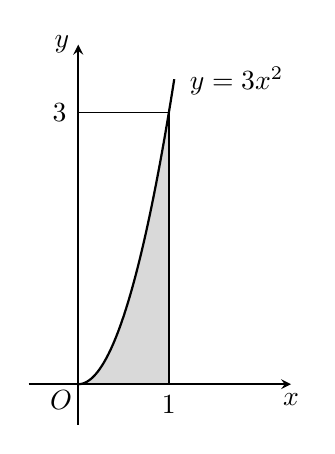
\begin{tikzpicture}[x=1.15cm, y=1.15cm, semithick, line join=round]

  % 阴影：曲线下方、x=1 左侧、x 轴上方
  \fill[gray!30] plot[domain=0:1, samples=60] (\x,{3*\x*\x}) -- (1,0) -- cycle;

  % 坐标轴
  \draw[->, >=stealth] (-0.55,0) -- (2.35,0) node[below, inner sep=3pt] {$x$};
  \draw[->, >=stealth] (0,-0.45) -- (0,3.75) node[left, inner sep=3pt] {$y$};

  % 长方形：y=3 的水平边、x=1 的竖直边
  \draw (0,3) -- (1,3);
  \draw (1,0) -- (1,3);

  % 抛物线 y=3x²（在 (1,3) 之外略向上延伸）
  \draw[thick, domain=0:1.06, samples=80] plot (\x,{3*\x*\x});
  \node[right] at (1.12,3.35) {$y=3x^2$};

  % 刻度与原点
  \node[below left, inner sep=2pt] at (0,0) {$O$};
  \node[below, inner sep=4pt] at (1,0) {$1$};
  \node[left, inner sep=4pt] at (0,3) {$3$};
\end{tikzpicture}
